% ============================================================
% Reporte: Ecuación de Optimalidad de Bellman en el Mundo del Wumpus
% Generado con "npm run report:latex" (scripts/report-latex.ts):
% todas las tablas y números provienen del mismo código del juego.
% Sube a Overleaf este archivo y la carpeta figuras/ (incluye ahí
% tu logo como figuras/logo_ibero.png).
% ============================================================
\documentclass[11pt,letterpaper]{article}

\usepackage[T1]{fontenc}
\usepackage[utf8]{inputenc}
\usepackage[spanish,es-tabla,es-nodecimaldot,es-noshorthands]{babel}
\usepackage{lmodern}
\usepackage[margin=2.5cm,headheight=14pt]{geometry}
\usepackage{amsmath,amssymb}
\usepackage{graphicx}
\usepackage{float}
\usepackage{booktabs}
\usepackage[table]{xcolor}
\usepackage{caption}
\usepackage{enumitem}
\usepackage{fancyhdr}
\usepackage{titlesec}
\usepackage{algorithm}
\usepackage{algpseudocode}
\usepackage[most]{tcolorbox}
\usepackage[hidelinks]{hyperref}

\definecolor{ibero}{HTML}{D52B1E}
\definecolor{oro}{HTML}{B8860B}

\titleformat{\section}{\Large\bfseries\color{ibero}}{\thesection}{0.6em}{}
\titleformat{\subsection}{\large\bfseries\color{ibero}}{\thesubsection}{0.6em}{}
\titleformat{\subsubsection}{\normalsize\bfseries}{\thesubsubsection}{0.6em}{}
\captionsetup{font=small,labelfont={bf,color=ibero}}

\pagestyle{fancy}
\fancyhf{}
\fancyhead[L]{\small Aprendizaje Reforzado}
\fancyhead[R]{\small Bellman en el Mundo del Wumpus}
\fancyfoot[C]{\small\thepage}
\renewcommand{\headrule}{{\color{ibero}\hrule height 0.6pt}}

\floatname{algorithm}{Algoritmo}
\renewcommand{\algorithmicrequire}{\textbf{Entrada:}}
\renewcommand{\algorithmicensure}{\textbf{Salida:}}

\newtcolorbox{nota}[1][]{colback=ibero!5,colframe=ibero,boxrule=0.6pt,arc=2pt,left=6pt,right=6pt,top=4pt,bottom=4pt,#1}

\newcommand{\juego}{\url{https://sebastiux.github.io/practicabelman/}}
\newcommand{\repo}{\url{https://github.com/sebastiux/practicabelman}}

\begin{document}

% ------------------------------------------------------------ Portada
\begin{titlepage}
\centering
\IfFileExists{figuras/logo_ibero.png}{\includegraphics[width=0.42\textwidth]{figuras/logo_ibero.png}}{\fbox{\parbox[c][2.5cm][c]{0.42\textwidth}{\centering Logo Ibero\\ \footnotesize(figuras/logo\_ibero.png)}}}\par
\vspace{1.2cm}
{\Large\bfseries Universidad Iberoamericana}\par
\vspace{0.2cm}
{\large Aprendizaje Reforzado}\par
\vspace{1.6cm}
{\color{ibero}\rule{\linewidth}{1.2pt}}\par
\vspace{0.5cm}
{\Huge\bfseries Seek \& Bellman}\par
\vspace{0.4cm}
{\LARGE Ecuación de Optimalidad de Bellman\\[2pt] en el Mundo del Wumpus}\par
\vspace{0.4cm}
{\color{ibero}\rule{\linewidth}{1.2pt}}\par
\vspace{0.8cm}
{\large Práctica: Definiciones MDPs y Ecuaciones de Bellman}\par
\vfill
\begin{tabular}{rl}
\textbf{Alumno:} & \textit{Nombre del alumno} \\
\textbf{Profesores:} & Dr. Alexandro López González \\
 & Mtro. Julio Caballero Mora \\
\textbf{Fecha:} & \today \\
\end{tabular}\par
\vspace{1cm}
{\small Juego: \juego\\ Código: \repo}
\end{titlepage}

\tableofcontents
\newpage

% ------------------------------------------------------------
\section{Introducción}

Un agente que toma decisiones en secuencia no debe maximizar la recompensa inmediata, sino la ganancia acumulada que recibirá a lo largo del episodio. Los Procesos de Decisión de Markov (MDP) formalizan este problema y las ecuaciones de Bellman permiten calcular qué tan bueno es cada estado relacionando su valor con el de los estados futuros, sin tener que observar todas las recompensas hasta el final.

En esta práctica se implementa la \textbf{Ecuación de Optimalidad de Bellman} ($V_*$) mediante el algoritmo de \textbf{iteración de valores} para encontrar la política óptima de navegación en un \emph{Mundo del Wumpus} de $10 \times 10$ estados. Para hacerlo más didáctico, la solución se presenta como un juego web, \emph{Seek \& Bellman}, con temática de Metallica: cinco escenarios inspirados en los discos \emph{Kill 'Em All}, \emph{Ride the Lightning}, \emph{Master of Puppets}, \emph{\ldots And Justice for All} y el \emph{Black Album}. En el juego se puede jugar manualmente, ver iteración por iteración cómo se propaga el valor y consultar el cálculo de la ecuación en cualquier celda.

\begin{nota}
\textbf{Juego en línea:} \juego\qquad \textbf{Código fuente:} \repo
\end{nota}

% ------------------------------------------------------------
\section{Objetivos}

\textbf{General.} Implementar la Ecuación de Optimalidad de Bellman para obtener $V_*$ y la política óptima $\pi_*$ de un agente que navega en el Mundo del Wumpus de $10\times10$, maximizando la ganancia acumulada y evitando los estados terminales negativos.

\textbf{Específicos.}
\begin{enumerate}[leftmargin=*]
  \item Modelar el ambiente como un MDP con estados, acciones, recompensas, tasa de descuento y transiciones.
  \item Implementar la iteración de valores con el criterio de paro $\Delta V < \varepsilon$.
  \item Explicar paso a paso cómo se propaga el valor iteración tras iteración y verificar que $V_*$ es punto fijo de la ecuación.
  \item Extraer la política óptima y comprobar que la ganancia de la trayectoria óptima coincide con $V_*(S_{0,0})$.
  \item Construir una herramienta interactiva que permita a cualquier estudiante comprender el funcionamiento de Bellman.
\end{enumerate}

% ------------------------------------------------------------
\section{Marco teórico}

\subsection{Procesos de Decisión de Markov}
Un MDP se define por un conjunto de estados $S$, un conjunto de acciones $A$, una dinámica $P(s', r \mid s, a)$ que da la probabilidad de llegar a $s'$ con recompensa $r$ al tomar la acción $a$ en el estado $s$, y una tasa de descuento $\gamma \in [0,1]$. Una \emph{política} $\pi(a \mid s)$ asigna a cada estado una probabilidad de tomar cada acción y sólo depende del estado actual.

\subsection{Ganancia y descuento}
El agente busca maximizar la ganancia esperada
\begin{equation}
G_t = R_{t+1} + \gamma R_{t+2} + \gamma^2 R_{t+3} + \cdots = \sum_{k=0}^{\infty} \gamma^k R_{t+k+1} = R_{t+1} + \gamma\, G_{t+1}.
\end{equation}
Si $\gamma = 0$ sólo importa la recompensa inmediata; conforme $\gamma \to 1$ el agente toma más en cuenta el futuro.

\subsection{Funciones de valor}
La función de valor estado bajo una política $\pi$ es la ganancia esperada al partir de $s$ y seguir $\pi$:
\begin{equation}
V_\pi(s) = \mathbb{E}_\pi\left[\, G_t \mid S_t = s \,\right], \qquad q_\pi(s,a) = \mathbb{E}_\pi\left[\, G_t \mid S_t = s, A_t = a \,\right].
\end{equation}

\subsection{Ecuaciones de Bellman}
Las ecuaciones de Bellman son recursivas: el valor de hoy es la recompensa inmediata más el valor descontado del mañana. Para evaluar una política:
\begin{equation}
V_\pi(s) = \sum_a \pi(a\mid s) \sum_{s',r} P(s',r \mid s,a)\,\big[r + \gamma V_\pi(s')\big].
\end{equation}
Para encontrar la política óptima, el promedio sobre las acciones se reemplaza por el máximo, lo que da la \textbf{Ecuación de Optimalidad de Bellman}:
\begin{equation}
\label{eq:optimalidad}
V_*(s) = \max_a \sum_{s',r} P(s',r \mid s,a)\,\big[r + \gamma V_*(s')\big].
\end{equation}

\subsection{Iteración de valores}
La ecuación~\eqref{eq:optimalidad} contiene a $V_*$ en ambos lados y un máximo, así que no se despeja directamente. La iteración de valores la convierte en una regla de actualización que se aplica a todos los estados en barridos sucesivos, a partir de $V_0 = 0$:
\begin{equation}
\label{eq:vi}
V_{k+1}(s) = \max_a \sum_{s',r} P(s',r \mid s,a)\,\big[r + \gamma V_k(s')\big], \qquad \Delta V_{k+1} = \max_s \big|V_{k+1}(s) - V_k(s)\big|.
\end{equation}
Para $\gamma < 1$ esta regla es una contracción y $V_k$ converge a $V_*$; se itera hasta que $\Delta V < \varepsilon$. Finalmente, la política óptima es la acción que alcanza el máximo:
\begin{equation}
\pi_*(s) = \arg\max_a \sum_{s',r} P(s',r \mid s,a)\,\big[r + \gamma V_*(s')\big].
\end{equation}

% ------------------------------------------------------------
\section{Planteamiento del problema}

\subsection{Definición del MDP}
\begin{table}[H]
\centering
\small
\caption{Definición del MDP de la práctica.}
\label{tab:mdp}
\begin{tabular}{ll}
\toprule
Elemento & Definición \\
\midrule
Estados $S$ & 100 celdas, $S_{0,0}$ a $S_{9,9}$ ($x$ = columna, $y$ = fila; $S_{0,0}$ abajo a la izquierda) \\
Acciones $A$ & Norte, Sur, Este y Oeste (un paso con distancia Manhattan) \\
Estado meta & $S_{9,9}$ (oro) con $r = +100$, terminal \\
Peligros & 20 pozos y 5 Wumpus distribuidos aleatoriamente, $r = -100$, terminales \\
Costo de vida & $r = -1$ por cada movimiento a una celda vacía \\
Fronteras & si la acción saca al agente de la red, permanece en $s$ con $r = -2$ \\
Descuento & $\gamma = 0.9$ \\
Convergencia & iterar hasta que $\Delta V < \varepsilon$, con $\varepsilon = 10^{-4}$ \\
Transiciones & deterministas: $P(s', r \mid s, a) = 1$ para el único $s'$ al que lleva $a$ \\
\bottomrule
\end{tabular}
\end{table}

Los estados terminales (oro, pozos y Wumpus) valen 0, porque al entrar en ellos termina el episodio; su recompensa se cobra en la transición que llega a ellos. Como las transiciones son deterministas, la suma sobre $s'$ y $r$ desaparece y la ecuación se simplifica a
\begin{equation}
\label{eq:det}
V_*(s) = \max_{a \in \{N,S,E,O\}} \big[\, r(s,a) + 0.9\, V_*(s') \,\big].
\end{equation}

\subsection{Escenarios del juego}
Cada disco es un escenario con la misma definición del MDP y una distribución distinta de peligros (semilla fija), con dificultad creciente: la ruta segura más corta de la entrada al oro mide de 18 a 26 pasos. Al generar el mapa se garantiza que exista al menos un camino seguro de $S_{0,0}$ al oro. El agente es un integrante de la banda y los peligros cambian de apariencia en cada disco (figura~\ref{fig:personajes}).

\begin{figure}[H]
\centering

\includegraphics[width=\textwidth]{figuras/fig_escenarios.png}
\caption{Selector de escenarios del juego: un nivel por disco.}
\label{fig:escenarios}
\end{figure}

\begin{figure}[H]
\centering

\includegraphics[width=0.95\textwidth]{figuras/fig_personajes.png}
\caption{Sprites pixel-art originales: agente, entrada, meta, percepciones y peligros de cada escenario.}
\label{fig:personajes}
\end{figure}

% ------------------------------------------------------------
\section{Implementación}

\subsection{Arquitectura}
El proyecto es una aplicación web en TypeScript (Vite + React) separada en dos capas:
\begin{itemize}[leftmargin=*]
  \item \textbf{Núcleo del MDP} (\texttt{src/core}), sin dependencias de la interfaz: generación del mundo con semilla (\texttt{world.ts}), modelo $P(s',r \mid s,a)$ con las recompensas de la práctica (\texttt{mdp.ts}) e iteración de valores, extracción de la política y simulación de trayectorias (\texttt{valueIteration.ts}).
  \item \textbf{Interfaz} (\texttt{src/components}): tablero, modo de juego, modo Bellman con inspector de la ecuación y gráfica de convergencia, y la explicación paso a paso calculada en vivo.
\end{itemize}
El sitio se publica automáticamente en GitHub Pages con GitHub Actions, que antes de cada despliegue ejecuta 30 pruebas automáticas del núcleo.

\subsection{Algoritmo}
La actualización se hace de forma \emph{síncrona}: $V_{k+1}$ se calcula usando sólo los valores de $V_k$, de modo que cada iteración se puede explicar de manera aislada.

\begin{algorithm}[H]
\caption{Iteración de valores (Ecuación de Optimalidad de Bellman)}
\label{alg:vi}
\begin{algorithmic}[1]
\Require MDP $(S, A, P, \gamma)$, umbral $\varepsilon$
\Ensure $V_*$ y $\pi_*$
\State $V(s) \gets 0$ para todo $s \in S$
\Repeat
  \State $V' \gets V$
  \For{cada estado no terminal $s$}
    \State $V'(s) \gets \max_a \sum_{s',r} P(s',r \mid s,a)\,[\,r + \gamma V(s')\,]$
  \EndFor
  \State $\Delta \gets \max_s |V'(s) - V(s)|$
  \State $V \gets V'$
\Until{$\Delta < \varepsilon$}
\State $\pi_*(s) \gets \arg\max_a \sum_{s',r} P(s',r \mid s,a)\,[\,r + \gamma V(s')\,]$
\State \Return $V$, $\pi_*$
\end{algorithmic}
\end{algorithm}

\subsection{Verificación}
Las pruebas automáticas comprueban, entre otras cosas, que el mundo tiene 20 pozos y 5 Wumpus con la entrada y el oro libres, que el choque con la frontera deja al agente en $s$ con $r=-2$, que un mundo de $3\times3$ resuelto a mano coincide con el algoritmo, que en los cinco escenarios $V_*$ es punto fijo de la ecuación (residual $\approx 0$) y que la política óptima llega al oro por la ruta más corta sin pisar peligros.

% ------------------------------------------------------------
\section{Resultados paso a paso (nivel 1: \emph{Kill 'Em All})}

El mapa del nivel 1 (semilla 1) tiene 20 pozos (charcos de sangre), 5 Wumpus (el Jinete), la entrada en $S_{0,0}$ y el oro en $S_{9,9}$. Quedan \textbf{74 estados no terminales} cuyo valor hay que calcular; los 26 terminales valen 0.

\begin{figure}[H]
\centering
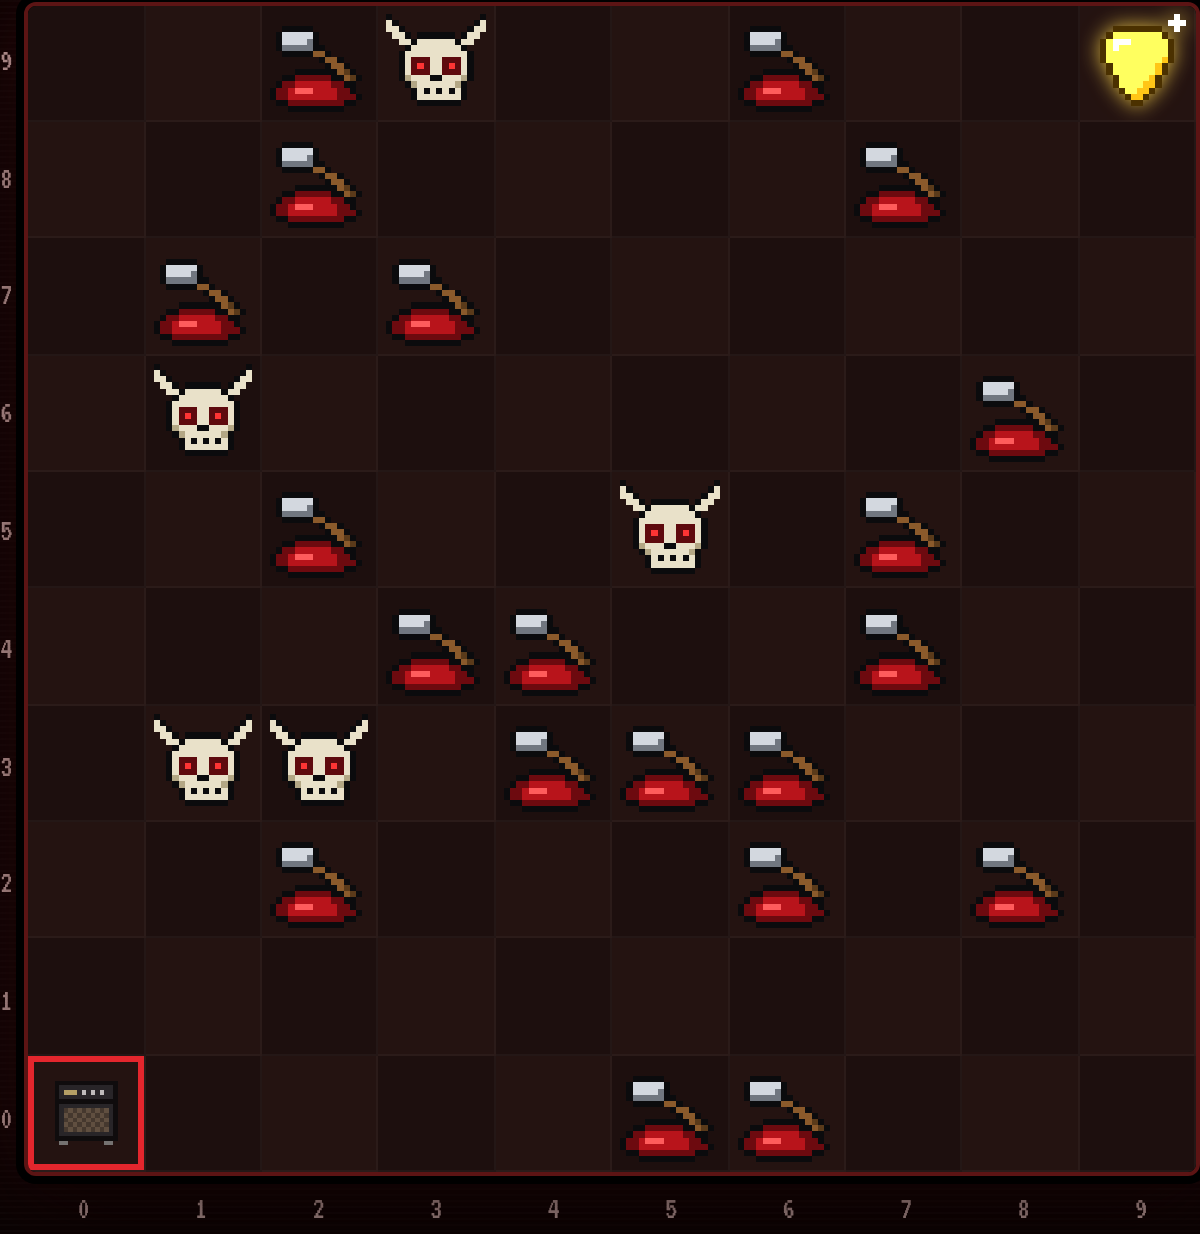
\includegraphics[width=0.55\textwidth]{figuras/fig_mapa.png}
\caption{Mapa del nivel 1. Abajo a la izquierda, la entrada $S_{0,0}$; arriba a la derecha, el oro $S_{9,9}$.}
\label{fig:mapa}
\end{figure}

\subsection{Paso 0: inicialización}
Se inicia con $V_0(s) = 0$ para los 100 estados. Por eso, en la primera iteración el término $\gamma V_0(s')$ vale 0 y sólo cuentan las recompensas inmediatas.

\subsection{Paso 1: primera iteración}
\paragraph{Vecino del oro ($S_{9,8}$).} Ir al Norte lleva al oro: $100 + 0.9\cdot 0 = 100$, que es el máximo.
\begin{table}[H]
\centering
\small
\caption{Cálculo de $V_1(S_{9,8})$, vecino del oro.}
\label{tab:it1-oro}
\begin{tabular}{lcrrr}
\toprule
Acción $a$ & $s'$ & $r$ & $V_{0}(s')$ & $r + \gamma\,V_{0}(s')$ \\
\midrule
Norte (N) & $S_{9,9}$ & $100$ & $0.00$ & $\mathbf{100.00}$ \\
Sur (S) & $S_{9,7}$ & $-1$ & $0.00$ & $-1.00$ \\
Este (E) & $S_{9,8}$ (borde) & $-2$ & $0.00$ & $-2.00$ \\
Oeste (O) & $S_{8,8}$ & $-1$ & $0.00$ & $-1.00$ \\
\bottomrule
\end{tabular}
\end{table}
\begin{align*}
Q(S_{9,8},N) &= 100 + 0.9\cdot(0.00) = 100.00 \\
Q(S_{9,8},S) &= -1 + 0.9\cdot(0.00) = -1.00 \\
Q(S_{9,8},E) &= -2 + 0.9\cdot(0.00) = -2.00 \\
Q(S_{9,8},O) &= -1 + 0.9\cdot(0.00) = -1.00 \\
V_{1}(S_{9,8}) &= \max\{100.00,\ -1.00,\ -2.00,\ -1.00\} = \mathbf{100.00}
\end{align*}

\paragraph{Junto a un peligro ($S_{2,1}$).} Entrar al charco de sangre vale $-100$; moverse a una celda vacía, $-1$. Gana moverse y el estado todavía no \emph{sabe} nada del oro.
\begin{table}[H]
\centering
\small
\caption{Cálculo de $V_1(S_{2,1})$, junto a un pozo.}
\label{tab:it1-peligro}
\begin{tabular}{lcrrr}
\toprule
Acción $a$ & $s'$ & $r$ & $V_{0}(s')$ & $r + \gamma\,V_{0}(s')$ \\
\midrule
Norte (N) & $S_{2,2}$ & $-100$ & $0.00$ & $-100.00$ \\
Sur (S) & $S_{2,0}$ & $-1$ & $0.00$ & $\mathbf{-1.00}$ \\
Este (E) & $S_{3,1}$ & $-1$ & $0.00$ & $\mathbf{-1.00}$ \\
Oeste (O) & $S_{1,1}$ & $-1$ & $0.00$ & $\mathbf{-1.00}$ \\
\bottomrule
\end{tabular}
\end{table}
\begin{align*}
Q(S_{2,1},N) &= -100 + 0.9\cdot(0.00) = -100.00 \\
Q(S_{2,1},S) &= -1 + 0.9\cdot(0.00) = -1.00 \\
Q(S_{2,1},E) &= -1 + 0.9\cdot(0.00) = -1.00 \\
Q(S_{2,1},O) &= -1 + 0.9\cdot(0.00) = -1.00 \\
V_{1}(S_{2,1}) &= \max\{-100.00,\ -1.00,\ -1.00,\ -1.00\} = \mathbf{-1.00}
\end{align*}

\paragraph{La entrada ($S_{0,0}$).} Es una esquina: Sur y Oeste chocan con la frontera ($-2$) y Norte y Este cuestan $-1$.
\begin{table}[H]
\centering
\small
\caption{Cálculo de $V_1(S_{0,0})$, esquina con dos fronteras.}
\label{tab:it1-entrada}
\begin{tabular}{lcrrr}
\toprule
Acción $a$ & $s'$ & $r$ & $V_{0}(s')$ & $r + \gamma\,V_{0}(s')$ \\
\midrule
Norte (N) & $S_{0,1}$ & $-1$ & $0.00$ & $\mathbf{-1.00}$ \\
Sur (S) & $S_{0,0}$ (borde) & $-2$ & $0.00$ & $-2.00$ \\
Este (E) & $S_{1,0}$ & $-1$ & $0.00$ & $\mathbf{-1.00}$ \\
Oeste (O) & $S_{0,0}$ (borde) & $-2$ & $0.00$ & $-2.00$ \\
\bottomrule
\end{tabular}
\end{table}
\begin{align*}
Q(S_{0,0},N) &= -1 + 0.9\cdot(0.00) = -1.00 \\
Q(S_{0,0},S) &= -2 + 0.9\cdot(0.00) = -2.00 \\
Q(S_{0,0},E) &= -1 + 0.9\cdot(0.00) = -1.00 \\
Q(S_{0,0},O) &= -2 + 0.9\cdot(0.00) = -2.00 \\
V_{1}(S_{0,0}) &= \max\{-1.00,\ -2.00,\ -1.00,\ -2.00\} = \mathbf{-1.00}
\end{align*}

Tras la primera iteración sólo los vecinos del oro valen 100; el resto de los estados no terminales vale $-1$, el costo de un paso (figura~\ref{fig:v1}).

\begin{figure}[H]
\centering
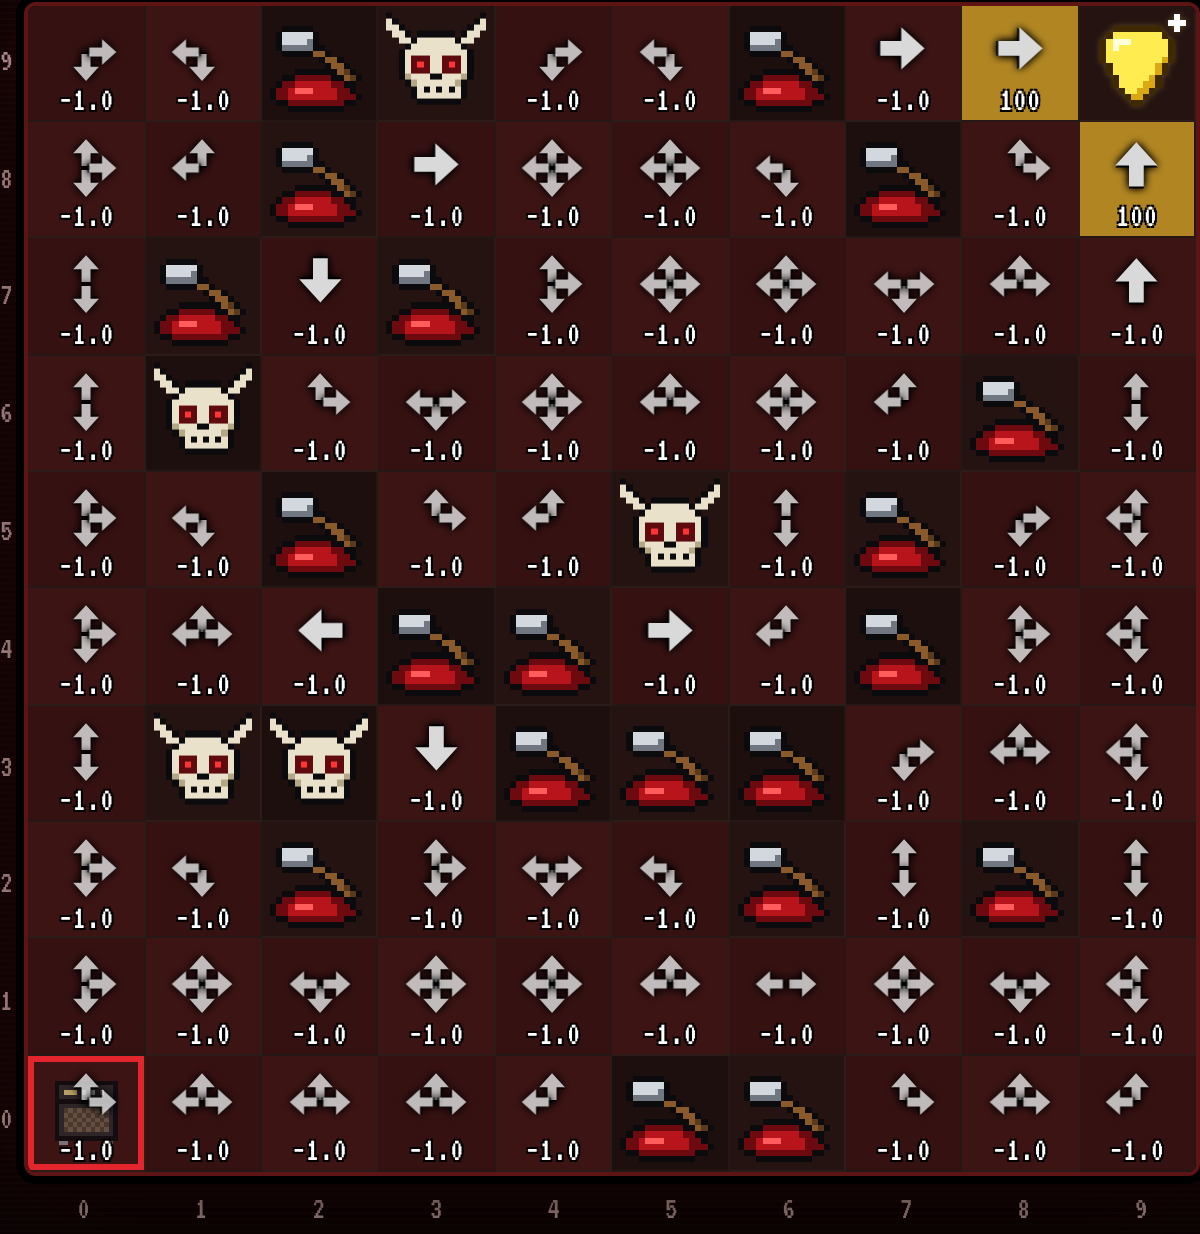
\includegraphics[width=0.6\textwidth]{figuras/fig_v1.png}
\caption{$V_1$: sólo los vecinos del oro tienen valor positivo. Las flechas muestran la acción greedy respecto a $V_1$; varias flechas pequeñas indican empate.}
\label{fig:v1}
\end{figure}

\subsection{Paso 2: segunda iteración}
\paragraph{A dos pasos del oro ($S_{9,7}$).} Su vecino ya vale $V_1 = 100$, así que moverse hacia él vale $-1 + 0.9 \cdot 100 = 89$.
\begin{table}[H]
\centering
\small
\caption{Cálculo de $V_2(S_{9,7})$, a dos pasos del oro.}
\label{tab:it2-dos}
\begin{tabular}{lcrrr}
\toprule
Acción $a$ & $s'$ & $r$ & $V_{1}(s')$ & $r + \gamma\,V_{1}(s')$ \\
\midrule
Norte (N) & $S_{9,8}$ & $-1$ & $100.00$ & $\mathbf{89.00}$ \\
Sur (S) & $S_{9,6}$ & $-1$ & $-1.00$ & $-1.90$ \\
Este (E) & $S_{9,7}$ (borde) & $-2$ & $-1.00$ & $-2.90$ \\
Oeste (O) & $S_{8,7}$ & $-1$ & $-1.00$ & $-1.90$ \\
\bottomrule
\end{tabular}
\end{table}
\begin{align*}
Q(S_{9,7},N) &= -1 + 0.9\cdot(100.00) = 89.00 \\
Q(S_{9,7},S) &= -1 + 0.9\cdot(-1.00) = -1.90 \\
Q(S_{9,7},E) &= -2 + 0.9\cdot(-1.00) = -2.90 \\
Q(S_{9,7},O) &= -1 + 0.9\cdot(-1.00) = -1.90 \\
V_{2}(S_{9,7}) &= \max\{89.00,\ -1.90,\ -2.90,\ -1.90\} = \mathbf{89.00}
\end{align*}

\paragraph{La entrada.} Sigue lejos del oro: lo mejor es pagar otro paso, $-1 + 0.9\cdot(-1) = -1.9$.
\begin{table}[H]
\centering
\small
\caption{Cálculo de $V_2(S_{0,0})$.}
\label{tab:it2-entrada}
\begin{tabular}{lcrrr}
\toprule
Acción $a$ & $s'$ & $r$ & $V_{1}(s')$ & $r + \gamma\,V_{1}(s')$ \\
\midrule
Norte (N) & $S_{0,1}$ & $-1$ & $-1.00$ & $\mathbf{-1.90}$ \\
Sur (S) & $S_{0,0}$ (borde) & $-2$ & $-1.00$ & $-2.90$ \\
Este (E) & $S_{1,0}$ & $-1$ & $-1.00$ & $\mathbf{-1.90}$ \\
Oeste (O) & $S_{0,0}$ (borde) & $-2$ & $-1.00$ & $-2.90$ \\
\bottomrule
\end{tabular}
\end{table}
\begin{align*}
Q(S_{0,0},N) &= -1 + 0.9\cdot(-1.00) = -1.90 \\
Q(S_{0,0},S) &= -2 + 0.9\cdot(-1.00) = -2.90 \\
Q(S_{0,0},E) &= -1 + 0.9\cdot(-1.00) = -1.90 \\
Q(S_{0,0},O) &= -2 + 0.9\cdot(-1.00) = -2.90 \\
V_{2}(S_{0,0}) &= \max\{-1.90,\ -2.90,\ -1.90,\ -2.90\} = \mathbf{-1.90}
\end{align*}

\begin{figure}[H]
\centering

\includegraphics[width=0.6\textwidth]{figuras/fig_v2.png}
\caption{$V_2$: la zona dorada creció una celda alrededor del oro.}
\label{fig:v2}
\end{figure}

\subsection{Paso 3: la onda de valor}
En cada barrido la información del oro avanza \textbf{exactamente una celda}: tras $k$ iteraciones la conocen los estados que están a $k$ pasos o menos por caminos seguros (figura~\ref{fig:onda}). Un estado a distancia $k$ que todavía no conoce el oro sólo acumula costo de vida, $V_{k-1}(s) = -\sum_{t=0}^{k-2}\gamma^t = -\frac{1-\gamma^{k-1}}{1-\gamma}$; en la iteración $k$ recibe el oro y pasa a valer $-\frac{1-\gamma^{k-1}}{1-\gamma} + 100\,\gamma^{k-1}$. La diferencia es exactamente
\begin{equation}
\Delta V_k = 100\,\gamma^{k-1},
\end{equation}
lo que explica la serie $100, 90, 81, 72.9, \ldots$ de la tabla~\ref{tab:deltas}.

\begin{figure}[H]
\centering
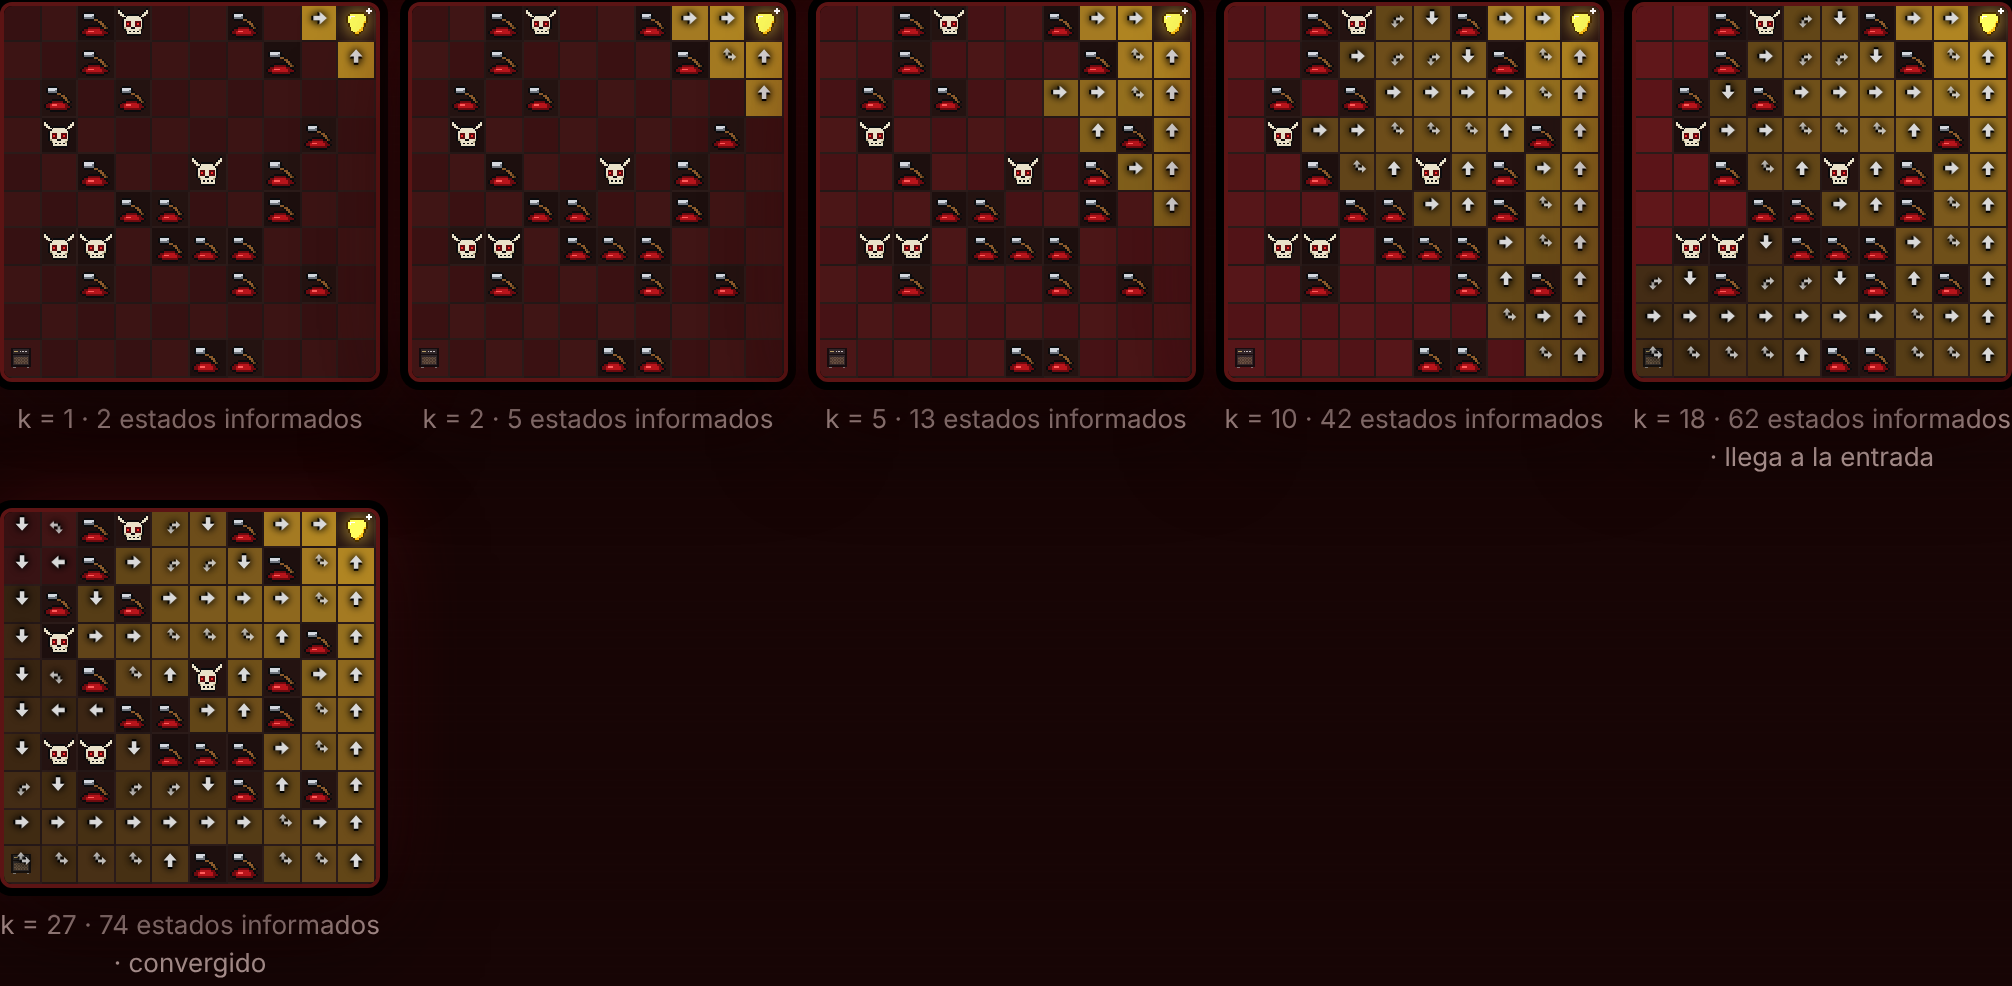
\includegraphics[width=\textwidth]{figuras/fig_onda.png}
\caption{Instantáneas de $V_k$ en $k = 1, 2, 5, 10, 18, 27$: la onda dorada crece una celda por iteración desde el oro.}
\label{fig:onda}
\end{figure}

\subsection{Paso 4: la entrada se entera del oro (\texorpdfstring{$k = 18$}{k = 18})}
La ruta segura más corta de $S_{0,0}$ al oro mide $d = 18$ pasos. Hasta la iteración 17 su mejor plan era vagar ($V_{17}(S_{0,0}) = -8.33$); en la iteración 18 su vecino sobre la ruta ya trae el valor del oro y $V_{18}(S_{0,0})$ salta a su valor definitivo (figura~\ref{fig:inspector}).
\begin{table}[H]
\centering
\small
\caption{Cálculo de $V_{18}(S_{0,0})$: el valor del oro llega a la entrada.}
\label{tab:aprende}
\begin{tabular}{lcrrr}
\toprule
Acción $a$ & $s'$ & $r$ & $V_{17}(s')$ & $r + \gamma\,V_{17}(s')$ \\
\midrule
Norte (N) & $S_{0,1}$ & $-1$ & $10.38$ & $\mathbf{8.34}$ \\
Sur (S) & $S_{0,0}$ (borde) & $-2$ & $-8.33$ & $-9.50$ \\
Este (E) & $S_{1,0}$ & $-1$ & $10.38$ & $\mathbf{8.34}$ \\
Oeste (O) & $S_{0,0}$ (borde) & $-2$ & $-8.33$ & $-9.50$ \\
\bottomrule
\end{tabular}
\end{table}
\begin{align*}
Q(S_{0,0},N) &= -1 + 0.9\cdot(10.38) = 8.34 \\
Q(S_{0,0},S) &= -2 + 0.9\cdot(-8.33) = -9.50 \\
Q(S_{0,0},E) &= -1 + 0.9\cdot(10.38) = 8.34 \\
Q(S_{0,0},O) &= -2 + 0.9\cdot(-8.33) = -9.50 \\
V_{18}(S_{0,0}) &= \max\{8.34,\ -9.50,\ 8.34,\ -9.50\} = \mathbf{8.34}
\end{align*}

\begin{figure}[H]
\centering
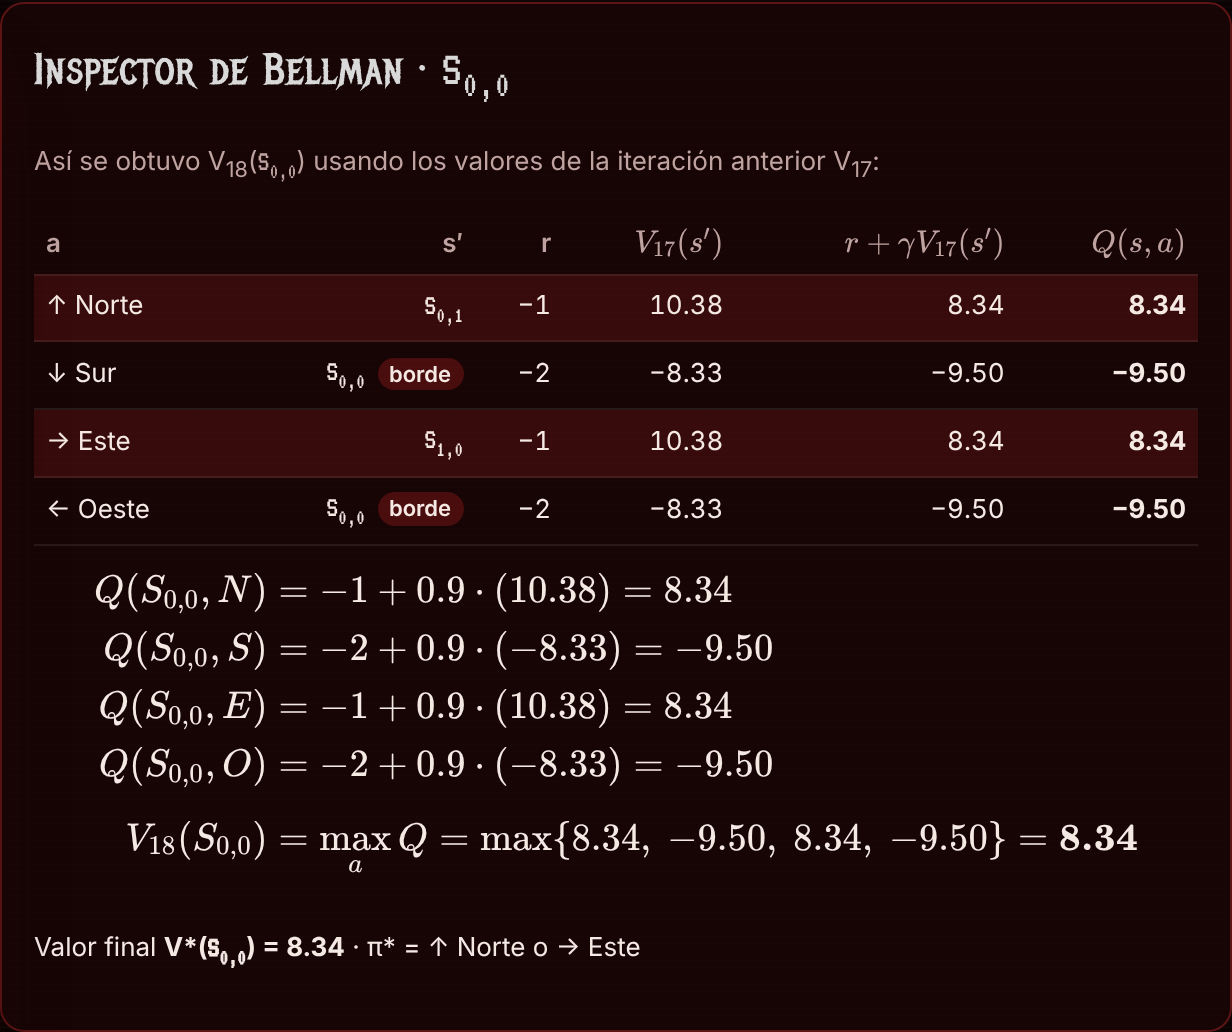
\includegraphics[width=0.6\textwidth]{figuras/fig_inspector.png}
\caption{Inspector de Bellman del juego en $k = 18$ para $S_{0,0}$.}
\label{fig:inspector}
\end{figure}

\subsection{Paso 5: convergencia}
El estado más lejano del oro está a $d_{\max} = 26$ pasos: recibe el valor del oro en la iteración 26 y en la iteración \textbf{$K = 27$} ya nada cambia ($\Delta V_{27} = 0.0000 < \varepsilon$), así que el algoritmo se detiene. En un MDP determinista como éste, la iteración de valores termina exactamente en $d_{\max} + 1$ barridos.

\begin{table}[H]
\centering
\footnotesize
\caption{Cambio máximo por iteración $\Delta V_k$, la ley $100\,\gamma^{k-1}$ y el número de estados que ya \emph{conocen} el oro ($d(s) \le k$).}
\label{tab:deltas}
\begin{tabular}{rrrr|rrrr}
\toprule
$k$ & $\Delta V_k$ & $100\gamma^{k-1}$ & inf. & $k$ & $\Delta V_k$ & $100\gamma^{k-1}$ & inf. \\
\midrule
1 & $100.0000$ & $100.0000$ & 2 & 15 & $22.8768$ & $22.8768$ & 54 \\
2 & $90.0000$ & $90.0000$ & 5 & 16 & $20.5891$ & $20.5891$ & 57 \\
3 & $81.0000$ & $81.0000$ & 7 & 17 & $18.5302$ & $18.5302$ & 60 \\
4 & $72.9000$ & $72.9000$ & 9 & 18 & $16.6772$ & $16.6772$ & 62 \\
5 & $65.6100$ & $65.6100$ & 13 & 19 & $15.0095$ & $15.0095$ & 63 \\
6 & $59.0490$ & $59.0490$ & 18 & 20 & $13.5085$ & $13.5085$ & 64 \\
7 & $53.1441$ & $53.1441$ & 24 & 21 & $12.1577$ & $12.1577$ & 66 \\
8 & $47.8297$ & $47.8297$ & 30 & 22 & $10.9419$ & $10.9419$ & 69 \\
9 & $43.0467$ & $43.0467$ & 38 & 23 & $9.8477$ & $9.8477$ & 70 \\
10 & $38.7420$ & $38.7420$ & 42 & 24 & $8.8629$ & $8.8629$ & 71 \\
11 & $34.8678$ & $34.8678$ & 45 & 25 & $7.9766$ & $7.9766$ & 73 \\
12 & $31.3811$ & $31.3811$ & 46 & 26 & $7.1790$ & $7.1790$ & 74 \\
13 & $28.2430$ & $28.2430$ & 48 & 27 & $0.0000$ & -- & 74 \\
14 & $25.4187$ & $25.4187$ & 51 &  & & &  \\
\bottomrule
\end{tabular}
\end{table}

\begin{figure}[H]
\centering
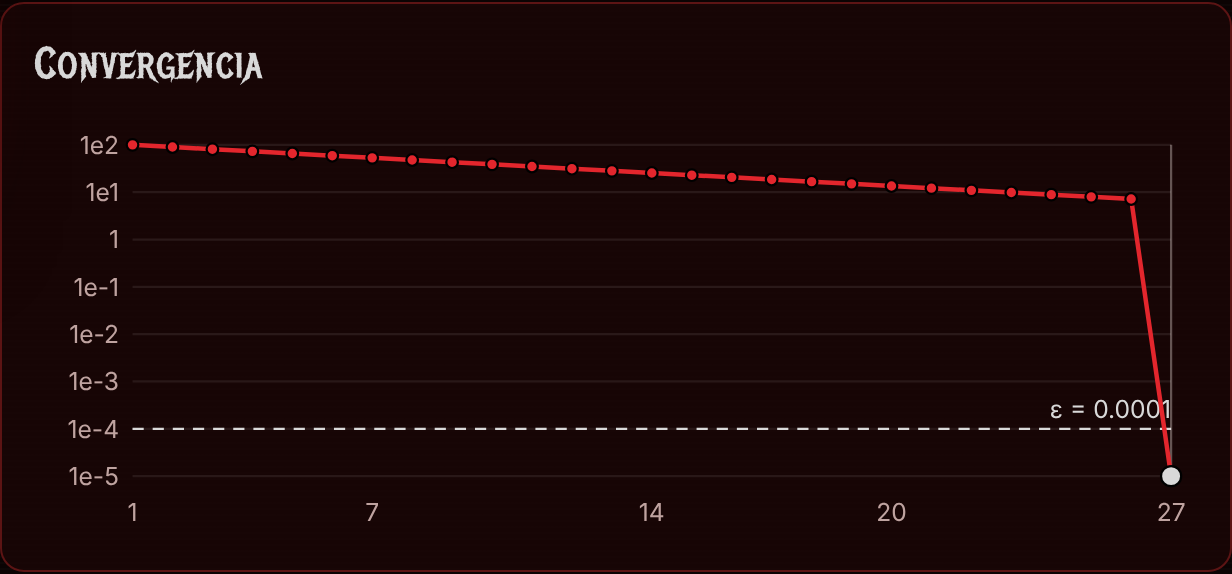
\includegraphics[width=0.65\textwidth]{figuras/fig_convergencia.png}
\caption{Convergencia: $\Delta V_k$ en escala logarítmica frente al umbral $\varepsilon = 10^{-4}$. La recta corresponde a $100\,\gamma^{k-1}$ y en $k = 27$ el cambio es 0.}
\label{fig:convergencia}
\end{figure}

\subsection{Paso 6: valores óptimos y política óptima}
Con $V_*$ convergido, la política óptima elige en cada estado la acción que alcanza el máximo. Ninguna flecha apunta a un peligro ni a la frontera: entrar a un pozo o con un Wumpus ($-100$) o chocar ($-2$ sin avanzar) siempre es peor que dar un paso de $-1$.

\begin{table}[H]
\centering
\footnotesize
\setlength{\tabcolsep}{3.5pt}
\caption{Valores óptimos $V_*(s)$ del nivel 1 (P = pozo, W = Wumpus, G = oro; los terminales valen 0).}
\label{tab:vstar}
\begin{tabular}{c|cccccccccc}
$y \backslash x$ & 0 & 1 & 2 & 3 & 4 & 5 & 6 & 7 & 8 & 9 \\
\hline
\textbf{9} & -1.2 & -2.1 & \textcolor{ibero}{P} & \textcolor{ibero}{\textbf{W}} & 37.4 & 42.6 & \textcolor{ibero}{P} & 89.0 & 100.0 & \textcolor{oro}{\textbf{G}} \\
\textbf{8} & -0.3 & -1.2 & \textcolor{ibero}{P} & 37.4 & 42.6 & 48.5 & 55.0 & \textcolor{ibero}{P} & 89.0 & 100.0 \\
\textbf{7} & 0.8 & \textcolor{ibero}{P} & 28.4 & \textcolor{ibero}{P} & 48.5 & 55.0 & 62.2 & 70.2 & 79.1 & 89.0 \\
\textbf{6} & 2.0 & \textcolor{ibero}{\textbf{W}} & 32.6 & 37.4 & 42.6 & 48.5 & 55.0 & 62.2 & \textcolor{ibero}{P} & 79.1 \\
\textbf{5} & 3.4 & 2.0 & \textcolor{ibero}{P} & 32.6 & 37.4 & \textcolor{ibero}{\textbf{W}} & 48.5 & \textcolor{ibero}{P} & 62.2 & 70.2 \\
\textbf{4} & 4.9 & 3.4 & 2.0 & \textcolor{ibero}{P} & \textcolor{ibero}{P} & 37.4 & 42.6 & \textcolor{ibero}{P} & 55.0 & 62.2 \\
\textbf{3} & 6.5 & \textcolor{ibero}{\textbf{W}} & \textcolor{ibero}{\textbf{W}} & 12.6 & \textcolor{ibero}{P} & \textcolor{ibero}{P} & \textcolor{ibero}{P} & 42.6 & 48.5 & 55.0 \\
\textbf{2} & 8.3 & 10.4 & \textcolor{ibero}{P} & 15.2 & 18.0 & 21.1 & \textcolor{ibero}{P} & 37.4 & \textcolor{ibero}{P} & 48.5 \\
\textbf{1} & 10.4 & 12.6 & 15.2 & 18.0 & 21.1 & 24.5 & 28.4 & 32.6 & 37.4 & 42.6 \\
\textbf{0} & 8.3 & 10.4 & 12.6 & 15.2 & 18.0 & \textcolor{ibero}{P} & \textcolor{ibero}{P} & 28.4 & 32.6 & 37.4 \\
\end{tabular}
\end{table}

\begin{table}[H]
\centering
\footnotesize
\setlength{\tabcolsep}{3.5pt}
\caption{Política óptima $\pi_*(s)$ del nivel 1. Dos flechas indican un empate: ambas acciones alcanzan el máximo.}
\label{tab:pistar}
\begin{tabular}{c|cccccccccc}
$y \backslash x$ & 0 & 1 & 2 & 3 & 4 & 5 & 6 & 7 & 8 & 9 \\
\hline
\textbf{9} & $\downarrow$ & $\downarrow\leftarrow$ & \textcolor{ibero}{P} & \textcolor{ibero}{\textbf{W}} & $\downarrow\rightarrow$ & $\downarrow$ & \textcolor{ibero}{P} & $\rightarrow$ & $\rightarrow$ & \textcolor{oro}{\textbf{G}} \\
\textbf{8} & $\downarrow$ & $\leftarrow$ & \textcolor{ibero}{P} & $\rightarrow$ & $\downarrow\rightarrow$ & $\downarrow\rightarrow$ & $\downarrow$ & \textcolor{ibero}{P} & $\uparrow\rightarrow$ & $\uparrow$ \\
\textbf{7} & $\downarrow$ & \textcolor{ibero}{P} & $\downarrow$ & \textcolor{ibero}{P} & $\rightarrow$ & $\rightarrow$ & $\rightarrow$ & $\rightarrow$ & $\uparrow\rightarrow$ & $\uparrow$ \\
\textbf{6} & $\downarrow$ & \textcolor{ibero}{\textbf{W}} & $\rightarrow$ & $\rightarrow$ & $\uparrow\rightarrow$ & $\uparrow\rightarrow$ & $\uparrow\rightarrow$ & $\uparrow$ & \textcolor{ibero}{P} & $\uparrow$ \\
\textbf{5} & $\downarrow$ & $\downarrow\leftarrow$ & \textcolor{ibero}{P} & $\uparrow\rightarrow$ & $\uparrow$ & \textcolor{ibero}{\textbf{W}} & $\uparrow$ & \textcolor{ibero}{P} & $\rightarrow$ & $\uparrow$ \\
\textbf{4} & $\downarrow$ & $\leftarrow$ & $\leftarrow$ & \textcolor{ibero}{P} & \textcolor{ibero}{P} & $\rightarrow$ & $\uparrow$ & \textcolor{ibero}{P} & $\uparrow\rightarrow$ & $\uparrow$ \\
\textbf{3} & $\downarrow$ & \textcolor{ibero}{\textbf{W}} & \textcolor{ibero}{\textbf{W}} & $\downarrow$ & \textcolor{ibero}{P} & \textcolor{ibero}{P} & \textcolor{ibero}{P} & $\rightarrow$ & $\uparrow\rightarrow$ & $\uparrow$ \\
\textbf{2} & $\downarrow\rightarrow$ & $\downarrow$ & \textcolor{ibero}{P} & $\downarrow\rightarrow$ & $\downarrow\rightarrow$ & $\downarrow$ & \textcolor{ibero}{P} & $\uparrow$ & \textcolor{ibero}{P} & $\uparrow$ \\
\textbf{1} & $\rightarrow$ & $\rightarrow$ & $\rightarrow$ & $\rightarrow$ & $\rightarrow$ & $\rightarrow$ & $\rightarrow$ & $\uparrow\rightarrow$ & $\rightarrow$ & $\uparrow$ \\
\textbf{0} & $\uparrow\rightarrow$ & $\uparrow\rightarrow$ & $\uparrow\rightarrow$ & $\uparrow\rightarrow$ & $\uparrow$ & \textcolor{ibero}{P} & \textcolor{ibero}{P} & $\uparrow\rightarrow$ & $\uparrow\rightarrow$ & $\uparrow$ \\
\end{tabular}
\end{table}

\begin{figure}[H]
\centering

\includegraphics[width=0.62\textwidth]{figuras/fig_vstar.png}
\caption{$V_*$ (número y color) y $\pi_*$ (flechas). Resaltada, la trayectoria del agente desde la entrada hasta el oro.}
\label{fig:vstar}
\end{figure}

\subsection{Paso 7: verificación del punto fijo}
Si se sustituye $V_*$ en el lado derecho de la ecuación en la entrada, el máximo debe devolver exactamente $V_*(S_{0,0})$:
\begin{table}[H]
\centering
\small
\caption{Ecuación de optimalidad evaluada con $V_*$ en $S_{0,0}$.}
\label{tab:verificacion}
\begin{tabular}{lcrrr}
\toprule
Acción $a$ & $s'$ & $r$ & $V_*(s')$ & $r + \gamma\,V_*(s')$ \\
\midrule
Norte (N) & $S_{0,1}$ & $-1$ & $10.38$ & $\mathbf{8.34}$ \\
Sur (S) & $S_{0,0}$ (borde) & $-2$ & $8.34$ & $5.51$ \\
Este (E) & $S_{1,0}$ & $-1$ & $10.38$ & $\mathbf{8.34}$ \\
Oeste (O) & $S_{0,0}$ (borde) & $-2$ & $8.34$ & $5.51$ \\
\bottomrule
\end{tabular}
\end{table}
El máximo es $8.3449 = V_*(S_{0,0})$, con empate entre Norte y Este. En los 74 estados no terminales, el residual máximo $\max_s |V_*(s) - \max_a Q_*(s,a)|$ es $0$: $V_*$ es punto fijo de la ecuación de optimalidad.

\subsection{Paso 8: trayectoria óptima}
Siguiendo $\pi_*$ desde $S_{0,0}$, el agente llega al oro en 18 pasos, la ruta segura más corta posible:

\begin{table}[H]
\centering
\footnotesize
\setlength{\tabcolsep}{4pt}
\caption{Trayectoria siguiendo $\pi_*$ desde la entrada. La ganancia acumulada final coincide con $V_*(S_{0,0})$.}
\label{tab:trayectoria}
\begin{tabular}{rcccrrrrr}
\toprule
$t$ & $s_t$ & $a_t$ & $s_{t+1}$ & $r_{t+1}$ & $\gamma^t$ & $\gamma^t r_{t+1}$ & $G$ acumulada & $V_*(s_t)$ \\
\midrule
0 & $S_{0,0}$ & Norte & $S_{0,1}$ & $-1$ & $1.0000$ & $-1.0000$ & $-1.0000$ & $8.3449$ \\
1 & $S_{0,1}$ & Este & $S_{1,1}$ & $-1$ & $0.9000$ & $-0.9000$ & $-1.9000$ & $10.3832$ \\
2 & $S_{1,1}$ & Este & $S_{2,1}$ & $-1$ & $0.8100$ & $-0.8100$ & $-2.7100$ & $12.6480$ \\
3 & $S_{2,1}$ & Este & $S_{3,1}$ & $-1$ & $0.7290$ & $-0.7290$ & $-3.4390$ & $15.1645$ \\
4 & $S_{3,1}$ & Este & $S_{4,1}$ & $-1$ & $0.6561$ & $-0.6561$ & $-4.0951$ & $17.9605$ \\
5 & $S_{4,1}$ & Este & $S_{5,1}$ & $-1$ & $0.5905$ & $-0.5905$ & $-4.6856$ & $21.0672$ \\
6 & $S_{5,1}$ & Este & $S_{6,1}$ & $-1$ & $0.5314$ & $-0.5314$ & $-5.2170$ & $24.5192$ \\
7 & $S_{6,1}$ & Este & $S_{7,1}$ & $-1$ & $0.4783$ & $-0.4783$ & $-5.6953$ & $28.3546$ \\
8 & $S_{7,1}$ & Norte & $S_{7,2}$ & $-1$ & $0.4305$ & $-0.4305$ & $-6.1258$ & $32.6163$ \\
9 & $S_{7,2}$ & Norte & $S_{7,3}$ & $-1$ & $0.3874$ & $-0.3874$ & $-6.5132$ & $37.3514$ \\
10 & $S_{7,3}$ & Este & $S_{8,3}$ & $-1$ & $0.3487$ & $-0.3487$ & $-6.8619$ & $42.6127$ \\
11 & $S_{8,3}$ & Norte & $S_{8,4}$ & $-1$ & $0.3138$ & $-0.3138$ & $-7.1757$ & $48.4585$ \\
12 & $S_{8,4}$ & Norte & $S_{8,5}$ & $-1$ & $0.2824$ & $-0.2824$ & $-7.4581$ & $54.9539$ \\
13 & $S_{8,5}$ & Este & $S_{9,5}$ & $-1$ & $0.2542$ & $-0.2542$ & $-7.7123$ & $62.1710$ \\
14 & $S_{9,5}$ & Norte & $S_{9,6}$ & $-1$ & $0.2288$ & $-0.2288$ & $-7.9411$ & $70.1900$ \\
15 & $S_{9,6}$ & Norte & $S_{9,7}$ & $-1$ & $0.2059$ & $-0.2059$ & $-8.1470$ & $79.1000$ \\
16 & $S_{9,7}$ & Norte & $S_{9,8}$ & $-1$ & $0.1853$ & $-0.1853$ & $-8.3323$ & $89.0000$ \\
17 & $S_{9,8}$ & Norte & $S_{9,9}$ & $100$ & $0.1668$ & $16.6772$ & $8.3449$ & $100.0000$ \\
\bottomrule
\end{tabular}
\end{table}

\begin{equation}
G_0 = \sum_{t=0}^{17} \gamma^t r_{t+1} = 1.000(-1) + 0.900(-1) + 0.810(-1) + \cdots + 0.1668(100) = 8.3449 = V_*(S_{0,0}).
\end{equation}
La ganancia descontada de la trayectoria coincide con el valor calculado por Bellman, como dicta la definición $V(s) = \mathbb{E}[G_t \mid S_t = s]$. La última columna muestra que $V_*(s_t)$ crece conforme el agente se acerca al oro: es lo que le falta por cobrar desde ese estado.

\subsection{Paso 9: interpretación con una fórmula cerrada}
Como el MDP es determinista y cada paso cuesta lo mismo, el valor óptimo de un estado sólo depende de $d(s)$, el número de pasos de su ruta segura más corta al oro: paga $-1$ durante $d-1$ pasos y cobra $+100$ en el paso $d$:
\begin{equation}
V_*(s) = \sum_{t=0}^{d-2} \gamma^t (-1) + \gamma^{d-1}(100) = -\frac{1-\gamma^{d-1}}{1-\gamma} + 100\,\gamma^{d-1} = -10 + 110\,(0.9)^{d-1}.
\end{equation}
La expresión decrece con $d$, así que maximizar $V_*$ es exactamente tomar la ruta segura más corta. Para la entrada, $d = 18$ y $V_*(S_{0,0}) = -10 + 110\,(0.9)^{17} = 8.3449$. La diferencia máxima entre la fórmula y la iteración de valores en todo el mapa es del orden de $10^{-14}$ (error de redondeo).

\begin{table}[H]
\centering
\scriptsize
\setlength{\tabcolsep}{3pt}
\caption{Fórmula cerrada $V_*(d) = -10 + 110\,(0.9)^{d-1}$ y número de estados a cada distancia $d$ del oro en el nivel 1.}
\label{tab:cerrada}
\begin{tabular}{lrrrrrrrrrrrrr}
\toprule
$d$ & 1 & 2 & 3 & 4 & 5 & 6 & 7 & 8 & 9 & 10 & 11 & 12 & 13 \\
\midrule
$V_*(d)$ & 100.00 & 89.00 & 79.10 & 70.19 & 62.17 & 54.95 & 48.46 & 42.61 & 37.35 & 32.62 & 28.35 & 24.52 & 21.07 \\
\# estados & 2 & 3 & 2 & 2 & 4 & 5 & 6 & 6 & 8 & 4 & 3 & 1 & 2 \\
\bottomrule
\end{tabular}

\vspace{4pt}
\begin{tabular}{lrrrrrrrrrrrrr}
\toprule
$d$ & 14 & 15 & 16 & 17 & 18 & 19 & 20 & 21 & 22 & 23 & 24 & 25 & 26 \\
\midrule
$V_*(d)$ & 17.96 & 15.16 & 12.65 & 10.38 & 8.34 & 6.51 & 4.86 & 3.37 & 2.04 & 0.83 & -0.25 & -1.23 & -2.10 \\
\# estados & 3 & 3 & 3 & 3 & 2 & 1 & 1 & 2 & 3 & 1 & 1 & 2 & 1 \\
\bottomrule
\end{tabular}
\end{table}

% ------------------------------------------------------------
\section{Resultados en los cinco escenarios}

\begin{table}[H]
\centering
\small
\caption{Resultados de la iteración de valores en los cinco escenarios (parámetros de la práctica).}
\label{tab:escenarios}
\begin{tabular}{rlrrrrrc}
\toprule
Nivel & Disco & Semilla & $d(S_{0,0})$ & $d_{\max}$ & $K$ & $V_*(S_{0,0})$ & Residual \\
\midrule
1 & \textit{Kill 'Em All} & 1 & 18 & 26 & 27 & $8.3449$ & $0$ \\
2 & \textit{Ride the Lightning} & 1109 & 20 & 28 & 29 & $4.8594$ & $0$ \\
3 & \textit{Master of Puppets} & 6942 & 22 & 26 & 27 & $2.0361$ & $0$ \\
4 & \textit{...And Justice for All} & 21491 & 24 & 30 & 31 & $-0.2508$ & $0$ \\
5 & \textit{Metallica (The Black Album)} & 13782 & 26 & 30 & 31 & $-2.1031$ & $0$ \\
\bottomrule
\end{tabular}
\end{table}

\begin{figure}[H]
\centering
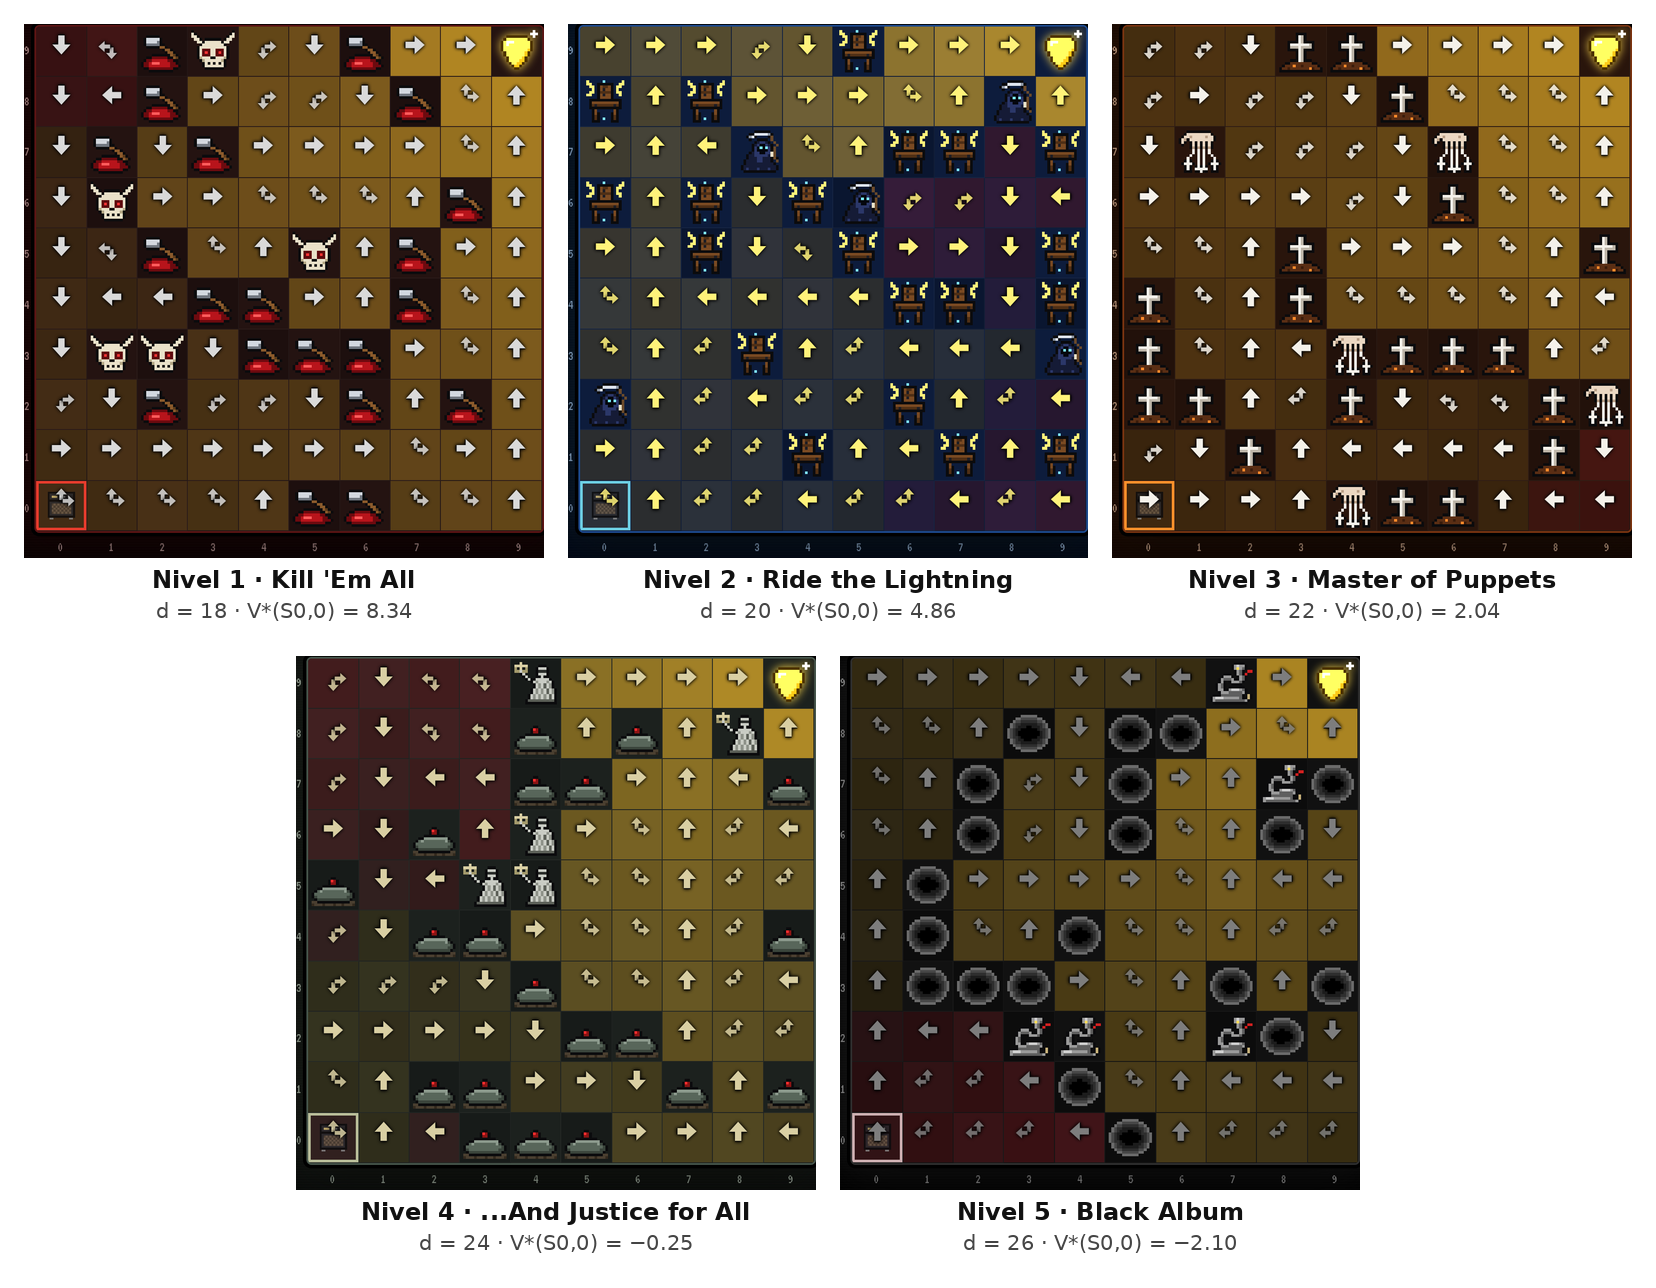
\includegraphics[width=\textwidth]{figuras/fig_niveles.png}
\caption{Valores y política óptima de los cinco niveles. Las flechas forman \emph{ríos} que fluyen hacia el oro rodeando los peligros.}
\label{fig:niveles}
\end{figure}

En todos los escenarios la iteración converge exactamente en $d_{\max}+1$ iteraciones, el residual de Bellman es 0 y la política óptima toma la ruta segura más corta. En los niveles 4 y 5 la ruta es tan larga ($d \ge 24$) que $V_*(S_{0,0})$ es negativo: el costo del camino supera al oro descontado. Aun así ir al oro sigue siendo óptimo, porque las alternativas son peores: vagar para siempre vale $\frac{-1}{1-\gamma} = -10$ y caer en un peligro, $-100$.

% ------------------------------------------------------------
\section{Análisis de sensibilidad}

El juego permite cambiar $\gamma$, $\varepsilon$ y agregar un \emph{resbalón}: con probabilidad $p$ el agente se mueve a una dirección perpendicular a la elegida ($p/2$ a cada lado), lo que vuelve estocástico al MDP. La tabla~\ref{tab:sensibilidad} resume el efecto en el nivel 1.

\begin{table}[H]
\centering
\small
\caption{Sensibilidad en el nivel 1: iteraciones $K$, valor de la entrada, estados cuya acción óptima cambia respecto a la práctica y resultados de 2000 episodios simulados siguiendo la política óptima de cada caso.}
\label{tab:sensibilidad}
\begin{tabular}{lrrrrr}
\toprule
Parámetros & $K$ & $V_*(S_{0,0})$ & cambios en $\pi_*$ & llega al oro & $\bar G$ simulado \\
\midrule
$\gamma = 0.5$ & 21 & $-2.00$ & 3 & $100.0\%$ & $-2.00$ \\
$\gamma = 0.7$ & 27 & $-3.09$ & 0 & $100.0\%$ & $-3.09$ \\
$\gamma = 0.9$ (práctica) & 27 & $8.34$ & 0 & $100.0\%$ & $8.34$ \\
$\gamma = 0.99$ & 27 & $68.59$ & 0 & $100.0\%$ & $68.59$ \\
$\varepsilon = 10^{-2}$ & 27 & $8.34$ & 0 & $100.0\%$ & $8.34$ \\
$\varepsilon = 10^{-6}$ & 27 & $8.34$ & 0 & $100.0\%$ & $8.34$ \\
resbalón $0.1$ & 89 & $-8.93$ & 9 & $73.7\%$ & $-8.09$ \\
resbalón $0.2$ & 89 & $-10.18$ & 14 & $0.1\%$ & $-10.16$ \\
\bottomrule
\end{tabular}
\end{table}

\begin{itemize}[leftmargin=*]
  \item \textbf{Descuento.} Con $\gamma = 0.99$ el agente valora mucho el futuro y $V_*(S_{0,0})$ sube a $68.59$; con $\gamma = 0.5$ el oro lejano casi no pesa y $V_*(S_{0,0}) = -2.00$, prácticamente el valor de vagar ($-1/(1-0.5) = -2$). En todos los casos el agente sigue llegando al oro por una ruta de 18 pasos; con $\gamma = 0.5$ sólo cambian 3 flechas por empates que se rompen distinto, porque los valores lejanos quedan casi iguales.
  \item \textbf{Umbral $\varepsilon$.} En el caso determinista no cambia el resultado: la iteración llega a $\Delta V = 0$ en $K = 27$.
  \item \textbf{Resbalón.} Con $p = 0.1$ la política cambia en 9 estados y llega al oro en el 73.7\% de los episodios. Con $p = 0.2$ caminar entre tantos peligros es tan riesgoso que la política óptima prefiere quedarse en zonas seguras ($V_*(S_{0,0}) = -10.18$). Si en ese mundo se usara la política determinista, el agente llegaría al oro sólo el 29.8\% de las veces y su ganancia media sería $-30.52$, mucho peor que $-10.16$. Además, la convergencia deja de ser exacta y $K$ depende de $\varepsilon$.
\end{itemize}

\begin{figure}[H]
\centering
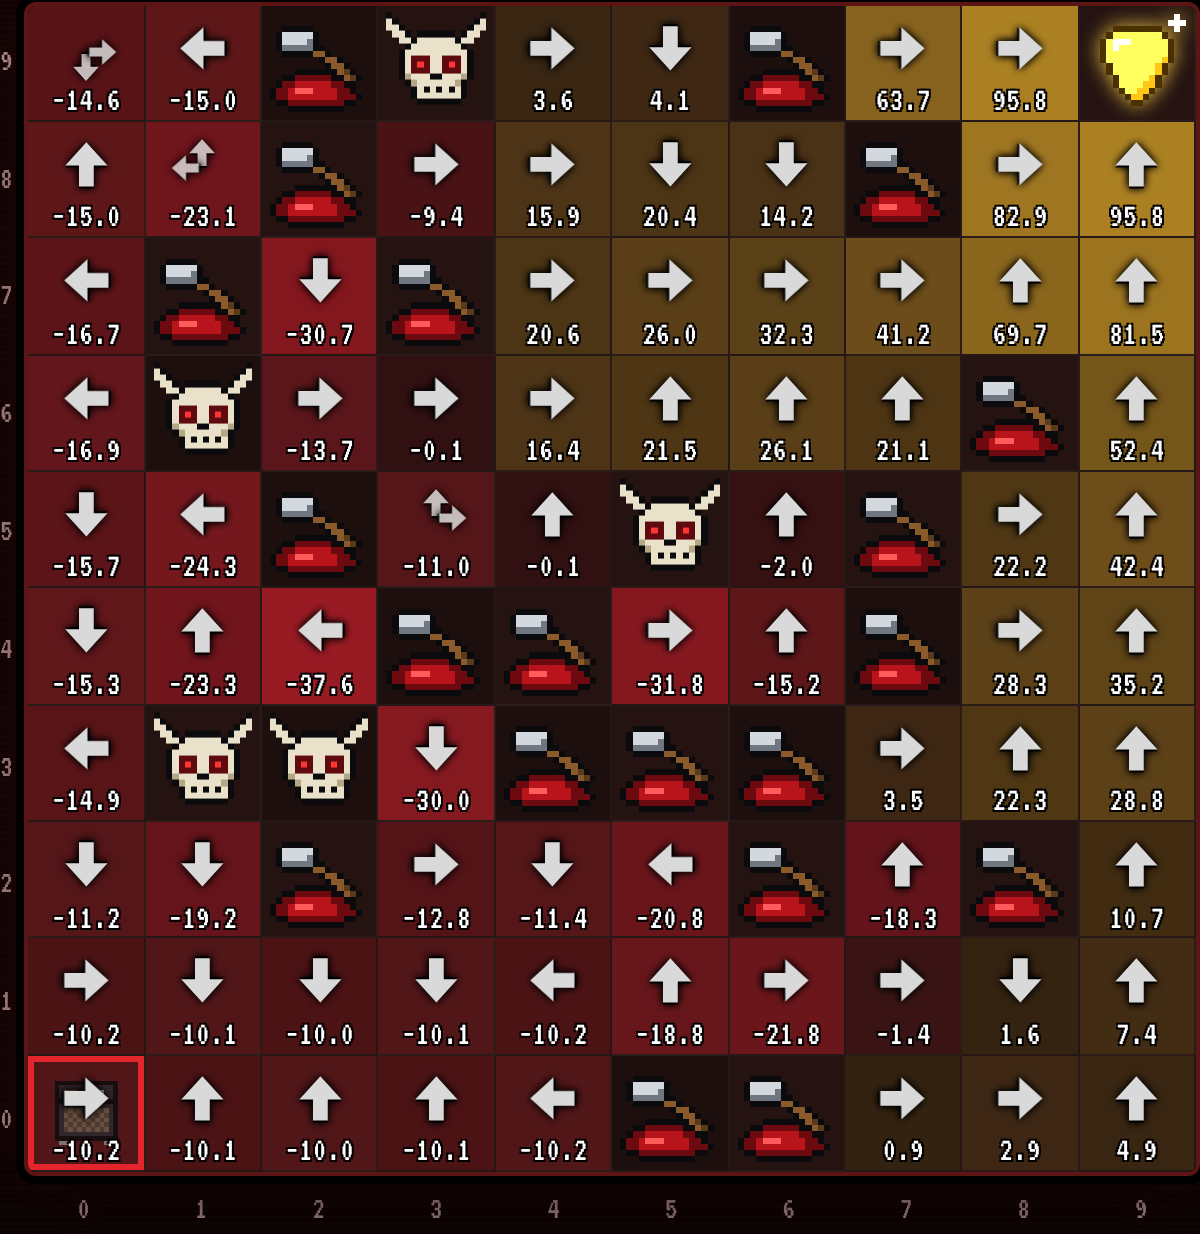
\includegraphics[width=0.55\textwidth]{figuras/fig_resbalon.png}
\caption{Política óptima con resbalón $p = 0.2$: cerca de la entrada el agente evita la zona de peligros.}
\label{fig:resbalon}
\end{figure}

% ------------------------------------------------------------
\section{Guía de juego paso a paso para estudiantes}

Esta guía está pensada para cualquier estudiante que quiera entender la Ecuación de Optimalidad de Bellman jugando. Sólo se necesita un navegador: \juego.

\subsection{Las reglas del mundo}
\begin{itemize}[leftmargin=*]
  \item Eres un integrante de la banda y empiezas en el amplificador, $S_{0,0}$ (esquina inferior izquierda). La meta es la púa de oro en $S_{9,9}$ (esquina superior derecha).
  \item Cada celda es un estado $S_{x,y}$ y las acciones son Norte, Sur, Este y Oeste.
  \item Cada paso a una celda vacía cuesta $-1$; chocar con el borde cuesta $-2$ y no te mueves; caer en un pozo o toparte con un Wumpus vale $-100$ y termina el juego; llegar al oro vale $+100$.
  \item Con $\gamma = 0.9$, una recompensa que llega dentro de $t$ pasos vale $\gamma^t$ veces su valor: el oro \emph{vale menos} mientras más tardes en llegar.
\end{itemize}

\subsection{Juega tú primero (pestaña \emph{Jugar})}
\begin{enumerate}[leftmargin=*]
  \item Elige un disco en la parte superior; empieza por \emph{Kill 'Em All} (nivel 1).
  \item Elige a tu integrante y muévete con las flechas, con W-A-S-D o con el control en pantalla. La tecla R reinicia.
  \item Hay niebla: sólo ves las celdas que ya visitaste. Usa las percepciones para deducir dónde están los peligros: \textbf{hedor} = hay un Wumpus al lado, \textbf{viento} = hay un pozo al lado, \textbf{brillo} = el oro está al lado.
  \item Observa el marcador: $\Sigma r$ es la suma simple de recompensas y $G = \sum_t \gamma^t r_{t+1}$ es la ganancia descontada, la cantidad que el agente quiere maximizar.
  \item Al terminar compara tu $G$ con $V_*(S_{0,0})$. Si tu $G$ es menor es porque diste pasos de más o te arriesgaste.
  \item Activa \emph{Consejo de Bellman} para ver la flecha de $\pi_*$ en tu celda, o \emph{Revelar el mapa} para ver todos los peligros.
\end{enumerate}

\begin{figure}[H]
\centering
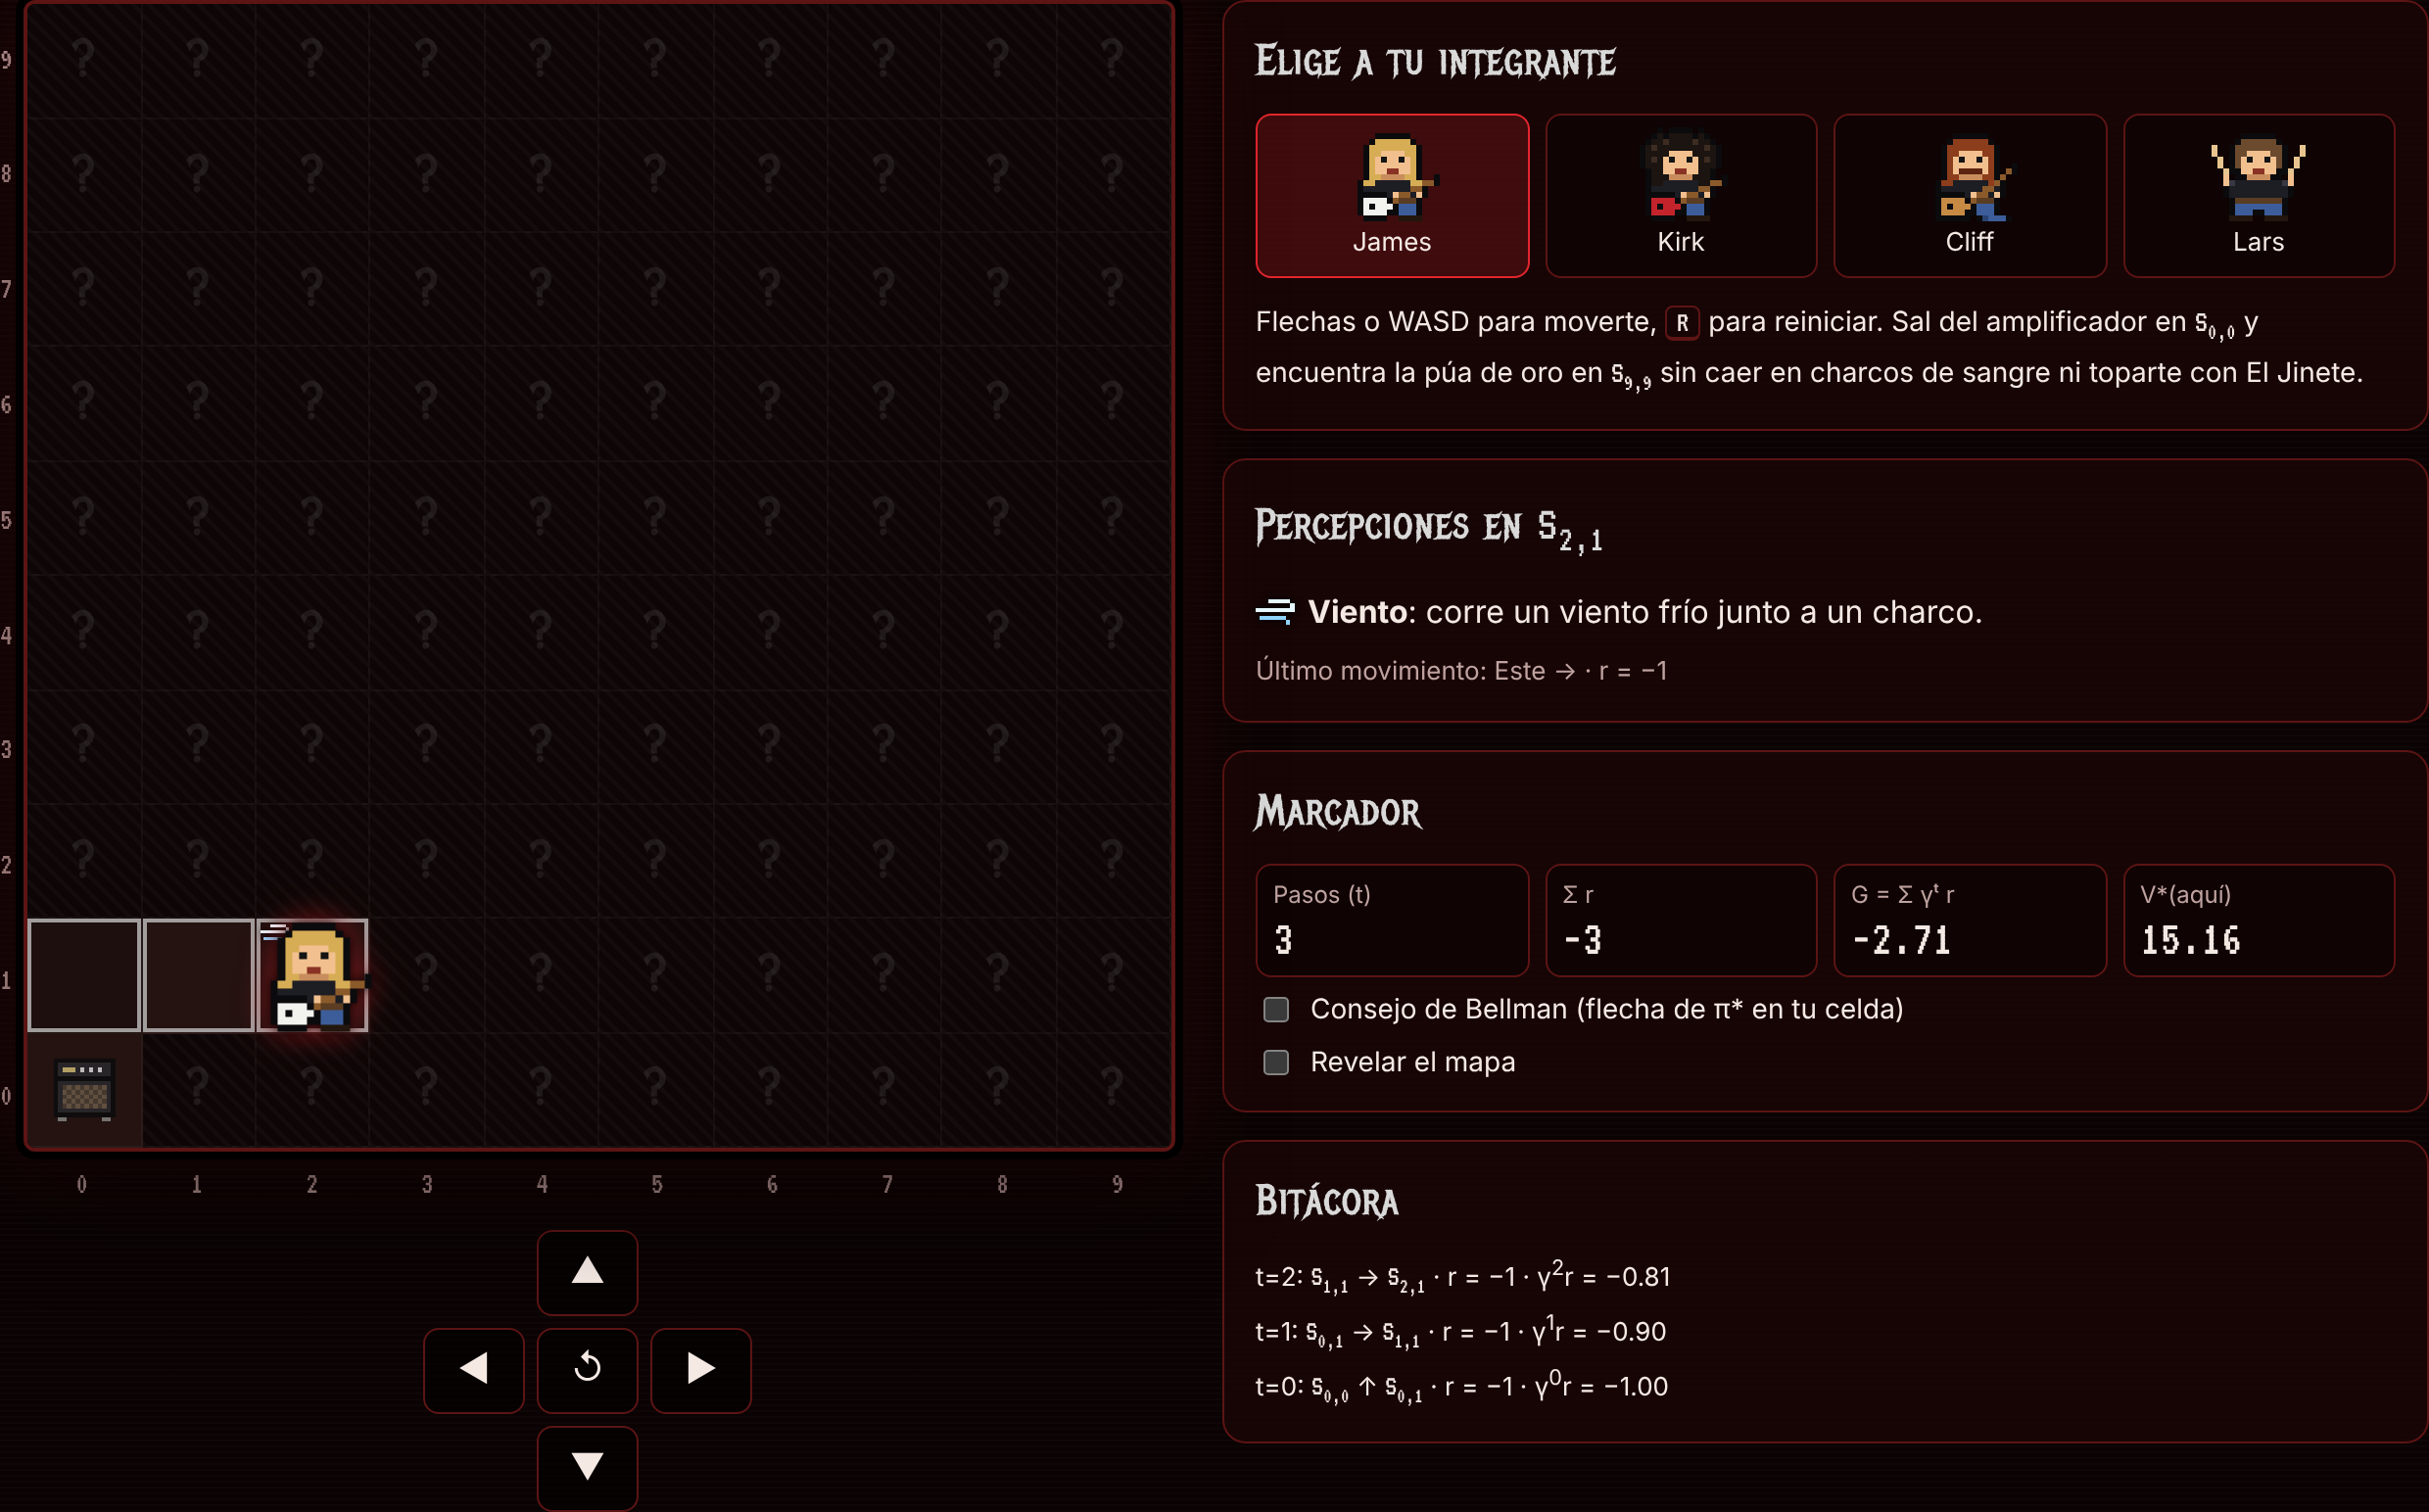
\includegraphics[width=0.95\textwidth]{figuras/fig_juego.png}
\caption{Modo de juego: niebla de guerra, percepción de viento junto a un pozo, marcador con $G$ y $V_*$, y bitácora con cada $\gamma^t r$.}
\label{fig:juego}
\end{figure}

\subsection{Mira cómo piensa Bellman (pestaña \emph{Bellman (IA)})}
\begin{enumerate}[leftmargin=*]
  \item Empiezas en $k = 0$: todos los valores valen $V_0 = 0$.
  \item Presiona el botón de siguiente iteración. En $k = 1$ sólo los vecinos del oro se vuelven dorados (valen 100) y el resto vale $-1$.
  \item Haz clic en $S_{9,8}$: el \emph{Inspector de Bellman} muestra $Q(S_{9,8},N) = 100 + 0.9\cdot 0 = 100$ y el máximo de las cuatro acciones.
  \item Avanza a $k = 2, 3, \ldots$: la zona dorada crece una celda por iteración ($89$, $79.1$, \ldots) y $\Delta V_k = 100, 90, 81, \ldots$
  \item Haz clic en $S_{0,0}$ y avanza: mientras el oro no llega su valor sólo acumula costo de vida ($-1$, $-1.9$, $-2.71$, \ldots) y en $k = d$ salta a su valor final.
  \item Presiona \emph{Iterar Bellman} para animar todo y observa la gráfica de convergencia: en la última iteración $\Delta V = 0 < \varepsilon$.
  \item Presiona \emph{Tocar $\pi_*$}: el agente sigue la política óptima y su $G$ coincide con $V_*(S_{0,0})$.
  \item Experimenta con $\gamma$ y con el resbalón en \emph{Parámetros del MDP} y explica qué cambia.
\end{enumerate}

\subsection{Lee la explicación (pestaña \emph{Explicación})}
Presenta, con los números del mapa elegido, el mismo desarrollo de la sección de resultados de este reporte: iteraciones desglosadas, onda de valor, convergencia, $V_*$, $\pi_*$, verificación y fórmula cerrada.

\subsection{Ejercicios sugeridos}
\begin{enumerate}[leftmargin=*]
  \item Calcula a mano $V_1$ y $V_2$ de una celda cualquiera y verifícalos con el inspector.
  \item Cuenta en el mapa los pasos $d$ de la entrada al oro, predice $V_*(S_{0,0}) = -10 + 110\,(0.9)^{d-1}$ y compáralo con el juego.
  \item En \emph{\ldots And Justice for All}, $V_*(S_{0,0})$ es negativo. ¿Por qué aun así conviene ir al oro?
  \item Con resbalón $0.2$, ¿qué celdas cambian de flecha y por qué?
\end{enumerate}

% ------------------------------------------------------------
\section{Conclusiones}
\begin{enumerate}[leftmargin=*]
  \item La iteración de valores aplica la Ecuación de Optimalidad de Bellman como regla de actualización y converge a $V_*$ en pocas decenas de iteraciones (27 en el nivel 1) con el criterio $\Delta V < \varepsilon$.
  \item El valor del oro se propaga desde $S_{9,9}$ como una onda, una celda por iteración, descontado por $\gamma$ y penalizado por el costo de vida; por eso $\Delta V_k = 100\gamma^{k-1}$ y $K = d_{\max} + 1$.
  \item La política óptima evita los 25 estados terminales negativos y las fronteras, y lleva de $S_{0,0}$ al oro por la ruta segura más corta: $V_*(s) = -10 + 110\,(0.9)^{d(s)-1}$.
  \item $V_*$ es punto fijo de la ecuación (residual 0) y coincide con la ganancia descontada de la trayectoria óptima, $G_0 = V_*(S_{0,0}) = 8.3449$.
  \item Cuando el ambiente es estocástico, la política óptima cambia: arriesgarse cerca de los peligros deja de valer la pena, lo que muestra que Bellman optimiza el valor \emph{esperado} y no sólo la ruta más corta.
\end{enumerate}

% ------------------------------------------------------------
\begin{thebibliography}{9}
\bibitem{sutton} R.~S. Sutton y A.~G. Barto, \emph{Reinforcement Learning: An Introduction}, 2.ª ed. Cambridge, MA: MIT Press, 2018.
\bibitem{bellman} R.~Bellman, \emph{Dynamic Programming}. Princeton, NJ: Princeton University Press, 1957.
\bibitem{russell} S.~Russell y P.~Norvig, \emph{Artificial Intelligence: A Modern Approach}, 4.ª ed. Pearson, 2021.
\bibitem{clase} A.~López González y J.~Caballero Mora, \emph{Aprendizaje reforzado: Definiciones MDPs}, Universidad Iberoamericana, notas del curso.
\end{thebibliography}

\end{document}
